 \let\negmedspace\undefined
\let\negthickspace\undefined
\documentclass[journal]{IEEEtran}
\usepackage[a5paper, margin=10mm, onecolumn]{geometry}
%\usepackage{lmodern} % Ensure lmodern is loaded for pdflatex
\usepackage{tfrupee} % Include tfrupee package

\setlength{\headheight}{1cm} % Set the height of the header box
\setlength{\headsep}{0mm}     % Set the distance between the header box and the top of the text
\usepackage{gvv-book}
\usepackage{gvv}
\usepackage{cite}
\usepackage{amsmath,amssymb,amsfonts,amsthm}
\usepackage{algorithmic}
\usepackage{graphicx}
\usepackage{textcomp}
\usepackage{xcolor}
\usepackage{txfonts}
\usepackage{listings}
\usepackage{enumitem}
\usepackage{mathtools}
\usepackage{gensymb}
\usepackage{comment}
\usepackage[breaklinks=true]{hyperref}
\usepackage{tkz-euclide} 
\usepackage{listings}
% \usepackage{gvv}                                        
\def\inputGnumericTable{}                                 
\usepackage[latin1]{inputenc}                                
\usepackage{color}                                            
\usepackage{array}                                            
\usepackage{longtable}                                       
\usepackage{calc}                                             
\usepackage{multirow}                                         
\usepackage{hhline}                                           
\usepackage{ifthen}                                           
\usepackage{lscape}



\usepackage{amsmath,amssymb}
\usepackage{booktabs}
\usepackage{tikz}
\usetikzlibrary{arrows.meta,angles,quotes}





\begin{document}

\bibliographystyle{IEEEtran}
\vspace{3cm}

\title{3.2.24}
\author{AI25BTECH11008 - Chiruvella Harshith Sharan}
% \maketitle
% \newpage
% \bigskip
{\let\newpage\relax\maketitle}

\renewcommand{\thefigure}{\theenumi}
\renewcommand{\thetable}{\theenumi}
\setlength{\intextsep}{10pt} % Space between text and floats


\numberwithin{equation}{enumi}
\numberwithin{figure}{enumi}
\renewcommand{\thetable}{\theenumi}


\textbf{Question:}
Construct a $\triangle ABC$ in which $CA = 6\,cm$, $AB = 5\,cm$, and $\angle BAC = 45^\circ$.
\vspace{0.3cm}

\textbf{Answer:}

\subsection*{\textbf{Step} 1: Define the coordinate system and vectors}

To solve the problem using vectors and matrices, place point $A$ at the origin of the coordinate system:

\[
\vec{A} = \begin{pmatrix}0 \\ 0\end{pmatrix}
\]

We want to find points $B$ and $C$ such that:

\[
|\vec{C} - \vec{A}| = 6, \quad |\vec{B} - \vec{A}| = 5, \quad \text{and} \quad \angle BAC = 45^\circ.
\]

\subsection*{\textbf{Step} 2: Position vector of point $B$}

Since $AB = 5\,cm$, and $\angle BAC = 45^\circ$, let us place $\vec{B}$ on the positive x-axis for convenience:

\[
\vec{B} = \begin{pmatrix}5 \\ 0\end{pmatrix}
\]

This choice sets the direction of $\vec{AB}$ along the x-axis.

\subsection*{\textbf{Step} 3: Position vector of point $C$}

Point $C$ must be at a distance of 6 from $A$ and must make a $45^\circ$ angle with vector $\vec{AB}$.

Using trigonometry, we can express $\vec{C}$ as:

\[
\vec{C} = 6 \begin{pmatrix} \cos 45^\circ \\ \sin 45^\circ \end{pmatrix} 
= 6 \begin{pmatrix} \frac{\sqrt{2}}{2} \\ \frac{\sqrt{2}}{2} \end{pmatrix}
= \begin{pmatrix} 3\sqrt{2} \\ 3\sqrt{2} \end{pmatrix}
\]

\subsection*{\textbf{Step} 4: Verification using dot product}

The angle $\theta$ between vectors $\vec{AB}$ and $\vec{AC}$ is given by:

\[
\cos \theta = \frac{(\vec{B}-\vec{A}) \cdot (\vec{C}-\vec{A})}{|\vec{B}-\vec{A}| \, |\vec{C}-\vec{A}|}
\]

Calculate:

\[
(\vec{B}-\vec{A}) \cdot (\vec{C}-\vec{A}) = \begin{pmatrix}5 \\ 0\end{pmatrix} \cdot \begin{pmatrix}3\sqrt{2} \\ 3\sqrt{2}\end{pmatrix} = 5 \times 3\sqrt{2} + 0 = 15\sqrt{2}
\]

Magnitudes:

\[
|\vec{B}-\vec{A}| = 5, \quad |\vec{C}-\vec{A}| = 6
\]

Therefore,

\[
\cos \theta = \frac{15\sqrt{2}}{5 \times 6} = \frac{15\sqrt{2}}{30} = \frac{\sqrt{2}}{2} = \cos 45^\circ
\]

This confirms the angle is $45^\circ$.

\subsection*{\textbf{Step} 5: Summary of points}

\[
\boxed{
\vec{A} = \begin{pmatrix}0 \\ 0\end{pmatrix}, \quad
\vec{B} = \begin{pmatrix}5 \\ 0\end{pmatrix}, \quad
\vec{C} = \begin{pmatrix}3\sqrt{2} \\ 3\sqrt{2}\end{pmatrix}
}
\]

These points construct the required triangle $\triangle ABC$ satisfying all given conditions.



\begin{figure}[htbp]
\centering
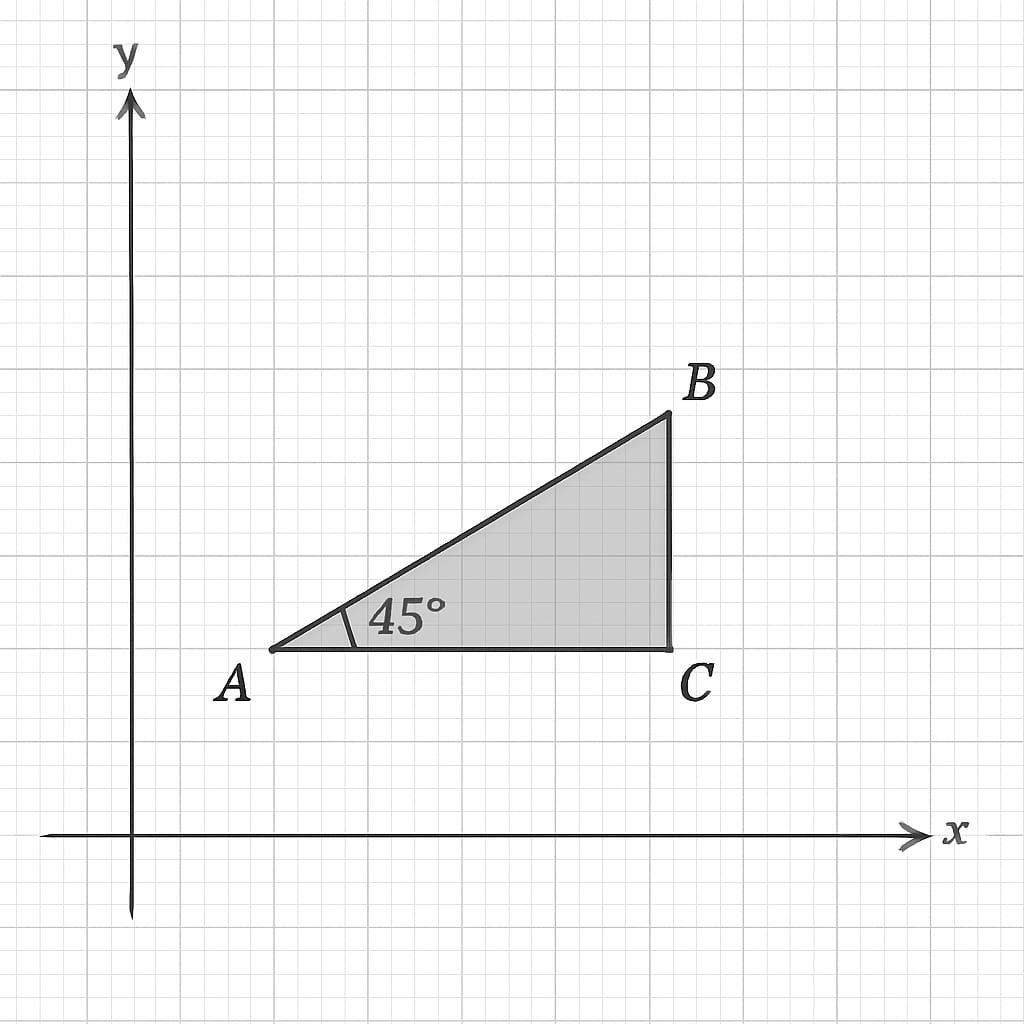
\includegraphics[width=0.7\columnwidth]{figs/fig1.png} 
\caption{plot}
\label{fig:1}
\end{figure}



\end{document}